

\documentclass{article}


\usepackage[left=1in,right=1in,top=1in,bottom=1in]{geometry}
\usepackage{wrapfig,subfig,graphicx}
\usepackage{latexsym,wasysym,amssymb,marvosym}
\usepackage{framed, color}
\definecolor{shadecolor}{RGB}{205,183,158}
\usepackage{multirow,booktabs}
\usepackage{soul}
\definecolor{navy}{RGB}{0,0,128}
\usepackage{float}
\floatstyle{boxed} 
\restylefloat{figure}

\newcommand{\mcomment}[1]{\textcolor{navy}{#1}}
\newcommand{\bigcheck}{\Large\CrossedBox}
\newcommand{\uncheck}{\Large\HollowBox}


\begin{document}
\renewcommand{\arraystretch}{1.1}


\section*{\LARGE{Montane Hardwood (MHW)}}

\begin{snugshade}\Large \textbf{General Information} \end{snugshade}

\subsection*{Crosswalks}
PNV Types:\\
%\begin{table}[!hbp]
%\begin{center}
%\footnotesize
\tiny 
\begin{tabular}{llllllll}
ABCO	&ABCO-PILA	&ABCO	&ABCO-PILA-PIJE	&PSME-MCN	&PSME-MCN-QUCH2	&n/a	&n/a\\
ABCO-MCN	&ABCO-MCN-LIDE3	&ABCO-MCN	&ABCO-MCN-LIDE2	&ABCO-MCN	&ABCO-MCN-LIDE3	&n/a	&n/a\\
ABCO-MCN	&ABCO-MCN-LIDE3	&ABCO-MCN	&ABCO-MCN-LIDE3	&ABCO-MCN	&ABCO-MCN-LIDE3	&n/a	&n/a\\
ABCO-MCN&	ABCO-MCN-LIDE3	&ABCO-MCN	&ABCO-MCN-LIDE3	&ABCO-MCN	&ABCO-MCN-QUCH2	&n/a	&n/a\\
ABCO-MCN	&	ABCO-MCN-LIDE3	&ABCO-MCN	&ABCO-MCN-LIDE3	&forb	forb&	n/a	&n/a\\
ABCO-MCN&	ABCO-MCN-LIDE3	&ABCO-MCN	&ABCO-MCN-LIDE3	&n/a	&n/a	&n/a&	n/a\\
ABCO-MCN&	ABCO-MCN-QUCH2 OR QUKE	&ABCO-MCN	&ABCO-MCN-QUCH2	&n/a&	n/a	&n/a	&n/a\\
ABCO-MCN	&	ABCO-MCN-QUKE	&ABCO-MCN	&ABCO-MCN-QUKE	&ABCO-MCN?	&ABCO-MCN-?	&n/a	&n/a\\
ABCO-MCN	&	ABCO-MCN-QUKE	&ABCO-MCN	&ABCO-MCN-QUKE	&PSME-MCN	&PSME-MCN-QUCH2	&n/a&	n/a\\
ABCO-MCN	&	ABCO-MCN-QUKE	&ABCO-MCN	&ABCO-MCN-QUKE	&PSME-MCN	&PSME-MCN-QUKE	&ABCO-MCN?	&ABCO-MCN-?\\
All	&All	&Riparian Herbaceous	&Various	&n/a&	n/a	&n/a	&n/a\\
%PIPO, PSME, PSME-mcn, ABCO	&Various	&Various	&Various	&ABCO-MCN	&ABCO-MCN-QUCH2	&n/a		&n/a\\
PSME-MCN	&PSME-MCN-QUCH2	&PSME-MCN	&PSME-MCN-QUCH	&ABCO-MCN?	&ABCO-MCN-?		&n/a		&n/a\\
PSME-MCN	&PSME-MCN-QUCH2	&PSME-MCN	&PSME-MCN-QUCH	&forb		&forb			&n/a		&n/a\\
PSME-MCN	&PSME-MCN-QUCH2	&PSME-MCN	&PSME-MCN-QUCH2	&ABCO-MCN	&ABCO-MCN-QUKE	&n/a		&n/a\\
PSME-MCN	&PSME-MCN-QUCH2	&PSME-MCN	&PSME-MCN-QUCH2	&ABCO-MCN	&ABCO-MCN-QUKE	&PSME-MCN	&PSME-MCN-QUCH\\
PSME-MCN	&PSME-MCN-QUCH2	&PSME-MCN	&PSME-MCN-QUCH2	&ABCO-MCN	&ABCO-MCN-QUKE	&PSME-MCN	&PSME-MCN-QUKE\\
PSME-MCN	&PSME-MCN-QUCH2	&PSME-MCN	&PSME-MCN-QUCH2	&forb		&forb			&n/a		&n/a\\
PSME-MCN	&PSME-MCN-QUCH2	&PSME-MCN	&PSME-MCN-QUCH2	&Various		&Various			&n/a		&n/a\\
\end{tabular}\\
%\end{center}
%\end{table}
\normalsize
Existing Veg Type: \\
%\begin{table}[!hbp]
%\begin{center}
\footnotesize

\begin{tabular}{llll}
White fir	&	Forest Land	&	White Fir	&	Black Oak	\\
Pacific Douglas-fir	&	Forest Land	&	Pacific Douglas-Fir	&	Canyon Live Oak	\\
Pacific Douglas-fir	&	Forest Land	&	Pacific Douglas-Fir	&	White Alder	\\
Pacific Douglas-fir	&	Forest Land	&	Pacific Douglas-Fir	&	Black Oak	\\
Pacific Douglas-fir	&	Forest Land	&	Pacific Douglas-Fir	&	Tanoak (Madrone)	\\
Sierra Nevada mixed conifer	&	Forest Land	&	Incense Cedar	&	Canyon Live Oak	\\
Sierra Nevada mixed conifer	&	Forest Land	&	Incense Cedar	&	Black Oak	\\
Sierra Nevada mixed conifer	&	Forest Land	&	Mixed Conifer - Pine	&	Interior Mixed Hardwood	\\
Sierra Nevada mixed conifer	&	Forest Land	&	Mixed Conifer - Pine	&	Canyon Live Oak	\\
Sierra Nevada mixed conifer	&	Forest Land	&	Mixed Conifer - Pine	&	White Alder	\\
Sierra Nevada mixed conifer	&	Forest Land	&	Mixed Conifer - Pine	&	Madrone	\\
Sierra Nevada mixed conifer	&	Forest Land	&	Mixed Conifer - Pine	&	Black Oak	\\
Sierra Nevada mixed conifer	&	Forest Land	&	Mixed Conifer - Pine	&	Tanoak (Madrone)	\\
Sierra Nevada mixed conifer	&	Forest Land	&	Mixed Conifer - Pine	&	Montane Mixed Hardwood	\\
Pacific ponderosa pine - Douglas-fir	&	Forest Land	&	Douglas-Fir - Ponderosa Pine	&	Riparian Mixed Hardwood	\\
Pacific ponderosa pine - Douglas-fir	&	Forest Land	&	Douglas-Fir - Ponderosa Pine	&	Canyon Live Oak	\\
Pacific ponderosa pine - Douglas-fir	&	Forest Land	&	Douglas-Fir - Ponderosa Pine	&	White Alder	\\
Pacific ponderosa pine - Douglas-fir	&	Forest Land	&	Douglas-Fir - Ponderosa Pine	&	Madrone	\\
Pacific ponderosa pine - Douglas-fir	&	Forest Land	&	Douglas-Fir - Ponderosa Pine	&	Black Oak	\\
Pacific ponderosa pine - Douglas-fir	&	Forest Land	&	Douglas-Fir - Ponderosa Pine	&	Tanoak (Madrone)	\\
Pacific ponderosa pine - Douglas-fir	&	Forest Land	&	Douglas-Fir - Ponderosa Pine	&	Montane Mixed Hardwood	\\
Pacific ponderosa pine	&	Forest Land	&	Ponderosa Pine	&	N/A	\\
Pacific ponderosa pine	&	Forest Land	&	Ponderosa Pine	&	Canyon Live Oak	\\
Pacific ponderosa pine	&	Forest Land	&	Ponderosa Pine	&	White Alder	\\
Pacific ponderosa pine	&	Forest Land	&	Ponderosa Pine	&	Madrone	\\
Pacific ponderosa pine	&	Forest Land	&	Ponderosa Pine	&	Black Oak	\\
Pacific ponderosa pine	&	Forest Land	&	Ponderosa Pine	&	Tanoak (Madrone)	\\
Pacific ponderosa pine	&	Forest Land	&	Ponderosa Pine	&	Willow - Alder	\\
Pacific ponderosa pine	&	Forest Land	&	Ponderosa Pine	&	Montane Mixed Hardwood	\\
California black oak	&	Forest Land	&	Madrone	&	N/A	\\
California black oak	&	Forest Land	&	Madrone	&	Wedgeleaf Ceanothus	\\
California black oak	&	Forest Land	&	Black Oak	&	N/A	\\
California black oak	&	Forest Land	&	Black Oak	&	Barren	\\
California black oak	&	Forest Land	&	Black Oak	&	Greenleaf Manzanita	\\
California black oak	&	Forest Land	&	Black Oak	&	Huckleberry Oak	\\
California black oak	&	Forest Land	&	Black Oak	&	Deerbrush	\\
California black oak	&	Forest Land	&	Black Oak	&	Scrub Oak	\\
California black oak	&	Forest Land	&	Black Oak	&	Whiteleaf Manzanita	\\
California black oak	&	Forest Land	&	Black Oak	&	Upper Montane Mixed Chaparral	\\
California black oak	&	Forest Land	&	Black Oak	&	Mountain Whitethorn	\\
California black oak	&	Forest Land	&	Black Oak	&	Eastside Pine	\\
California black oak	&	Forest Land	&	Black Oak	&	Perennial Grasses and Forbs	\\
California black oak	&	Forest Land	&	Black Oak	&	Mixed Conifer - Pine	\\
California black oak	&	Forest Land	&	Black Oak	&	Ponderosa Pine	\\
California black oak	&	Forest Land	&	Tanoak (Madrone)	&	N/A	\\
California black oak	&	Forest Land	&	Tanoak (Madrone)	&	Deerbrush	\\
California black oak	&	Forest Land	&	Tanoak (Madrone)	&	Wedgeleaf Ceanothus	\\
California black oak	&	Forest Land	&	Tanoak (Madrone)	&	Whiteleaf Manzanita	\\
California black oak	&	Forest Land	&	Tanoak (Madrone)	&	Mixed Conifer - Pine	\\
California black oak	&	Forest Land	&	Tanoak (Madrone)	&	Ponderosa Pine	\\
California black oak	&	Forest Land	&	Montane Mixed Hardwood	&	N/A	\\
California black oak	&	Forest Land	&	Montane Mixed Hardwood	&	Greenleaf Manzanita	\\
California black oak	&	Forest Land	&	Montane Mixed Hardwood	&	Deerbrush	\\
California black oak	&	Forest Land	&	Montane Mixed Hardwood	&	Wedgeleaf Ceanothus	\\
California black oak	&	Forest Land	&	Montane Mixed Hardwood	&	Lower Montane Mixed Chaparral	\\
California black oak	&	Forest Land	&	Montane Mixed Hardwood	&	Whiteleaf Manzanita	\\
Canyon live oak	&	Forest Land	&	Canyon Live Oak	&	N/A	\\
Canyon live oak	&	Forest Land	&	Canyon Live Oak	&	Greenleaf Manzanita	\\
Canyon live oak	&	Forest Land	&	Canyon Live Oak	&	Deerbrush	\\
Canyon live oak	&	Forest Land	&	Canyon Live Oak	&	Wedgeleaf Ceanothus	\\
Canyon live oak	&	Forest Land	&	Canyon Live Oak	&	Lower Montane Mixed Chaparral	\\
Canyon live oak	&	Forest Land	&	Canyon Live Oak	&	Scrub Oak	\\
Canyon live oak	&	Forest Land	&	Canyon Live Oak	&	Whiteleaf Manzanita	\\
Canyon live oak	&	Forest Land	&	Canyon Live Oak	&	Perennial Grasses and Forbs	\\
California coast live oak	&	Forest Land	&	Interior Mixed Hardwood	&	N/A	\\
	&		&		&		\\
White fir	&	Forest Land	&	Mixed Conifer - Fir	&	Black Oak	\\
White fir	&	Forest Land	&	White Fir	&	Canyon Live Oak	\\
\end{tabular}\\
%\end{center}
%\end{table}
\normalsize

\mcomment{EVeg not distinguished from TYPE at this time.}\\
Wieslander Veg Strings:
\par	Abies concolor--Pseudotsuga menziesii menziesii
\par	Arbutus menziesii
\par	Arbutus menziesii--Pteridium aquilinum pubescens
\par	Arbutus menziesii--Quercus kelloggii
\par	Lithocarpus densiflorus echinoides
\par	Lithocarpus densiflorus echinoides--Arctostaphylos patula
\par	Lithocarpus densiflorus echinoides--Pteridium aquilinum pubescens
\par	Lithocarpus densiflorus echinoides--Quercus kelloggii
\par	Lithocarpus densiflorus echinoides--Quercus vaccinifolia
\par	Lithocarpus densiflorus
\par	Lithocarpus densiflorus--Arbutus menziesii
\par	Quercus chrysolepis nana--Annuals
\par	Quercus chrysolepis
\par	Quercus chrysolepis--Aesculus californica
\par	Quercus chrysolepis--Aesculus californica--Vulpia myuros hirsuta
\par	Quercus chrysolepis--Arctostaphylos viscida
\par	Quercus chrysolepis--Arctostaphylos viscida--Bromus diandrus
\par	Quercus chrysolepis--Ceanothus cuneatus
\par	Quercus chrysolepis--Ceanothus cuneatus--Grass sp.
\par	Quercus chrysolepis--Ceanothus integerrimus
\par	Quercus chrysolepis--Ceanothus integerrimus--Ceanothus cuneatus
\par	Quercus chrysolepis--Chamaebatia foliolosa
\par	Quercus chrysolepis--Chamaebatia foliolosa--Grass sp.
\par	Quercus chrysolepis--Grass sp.
\par	Quercus chrysolepis--Pinus sabiniana
\par	Quercus chrysolepis--Pseudotsuga menziesii menziesii
\par	Quercus chrysolepis--Pseudotsuga menziesii menziesii--Abies concolor
\par	Quercus chrysolepis--Quercus douglasii--Ceanothus cuneatus--Grass sp.
\par	Quercus chrysolepis--Quercus kelloggii
\par	Quercus chrysolepis--Quercus kelloggii--Arctostaphylos viscida
\par	Quercus chrysolepis--Quercus kelloggii--Ceanothus integerrimus
\par	Quercus chrysolepis--Quercus kelloggii--Ceanothus integerrimus--Ceanothus cuneatus
\par	Quercus chrysolepis--Quercus kelloggii--Chamaebatia foliolosa
\par	Quercus chrysolepis--Quercus kelloggii--Chamaebatia foliolosa--Ceanothus integerrimus
\par	Quercus chrysolepis--Quercus kelloggii--Pseudotsuga menziesii menziesii--Pinus ponderosa
\par	Quercus chrysolepis--Quercus vaccinifolia
\par	Quercus chrysolepis--Quercus wislizeni--Arctostaphylos viscida--Heteromeles arbutifolia
\par	Quercus chrysolepis--Quercus wislizeni--Grass sp.--Ceanothus cuneatus
WHR Type: Montane Hardwood\\
BpS Model: 0610430 Mediterranean California Mixed Evergreen Forest (shared with DFTO) \\
\mcomment{Fire return intervals and high/low severity proportions were all calculated based on the BpS model and may need to be adjusted to be specific to the YHR type.}


%\paragraph{\large{Vegetation Description}} 
\subsection*{Vegetation Description}

\mcomment{Do we want to use common or scientific names, or both?}
\par A typical montane hardwood habitat is composed of a pronounced hardwood tree layer, with an infrequent and poorly developed shrub stratum, and a sparse herbaceous layer. On better sites, individual trees or clumps of trees may be only 3 to 4 m (10 to 13 ft) apart. On poorer sites, spacing increases to 8 to 10 m (26 to 33 ft). Where trees are closely spaced, crowns may close but seldom overlap. Living crowns on mature canyon live oaks occupy about 60 percent of the bole on typical sites and up to 80 percent on poor sites. %Tree heights tend to be uniform at most ages in mature stands where hardwoods occur, but subordinate to conifers. Mature oaks on better sites and in canyons range between 17 and 30 m (56 and 98 fl) tall and up to 150 cm (59) in) dbh. On poorer sites, mature trees typically are 10 to 15 m (33 to 49 ft) tall with boles up to 65 cm (26 in) in dbh, with dome-shaped crowns almost as wide as the trees are tall.
On rocky summits, canyon live oak is a shrub of small diameter, usually less than 4 m (13 ft) in height. Snags and downed woody material generally are sparse throughout the montane hardwood habitat. (WHR)

This type is characterized by the combination of coniferous and broadleaved trees. Characteristic trees include \emph{Pseudotsuga menziesii}, \emph{Quercus chrysolepis}, \emph{Lithocarpus densiflorus}, \emph{Arbutus menziesii}, \emph{Umbellularia californica}, \emph{Chrysolepis chrysophylla}. Species composition is primarily determined by the environmental gradients of temperature and moisture availability. Black oak (\emph{Quercus kelloggii}) is found on drier sites. Sugar pine (Pinus lambertiana) and ponderosa pine can be present in this type. Western hemlock can be the over-topping conifer, and understory species may include \emph{Acer macrophyllum}, \emph{Polystichum munitum} and \emph{Oxalis oregana}. (BPS)

These stands tend to have dense, or diverse shrub understories with \emph{Corylus cornuta}, \emph{Vaccinium ovatum}, \emph{Rhododendron macrophyllum}, \emph{Gaultheria shallon} and \emph{Toxicodendron diversilobum} being common. (BPS)

Steep, rocky south slopes of major river canyons often are clothed extensively by canyon live oak and scattered old-growth Douglas-fir. Elsewhere, higher elevation overstory associates are typical mixed conifer and California black oak; lower elevation associates are foothill pine, knobcone pine, tanoak, Pacific madrone, and scrubby California-laurel. (WHR)

These stands tend to have dense, or diverse shrub understories with \emph{Corylus cornuta}, \emph{Vaccinium ovatum}, \emph{Rhododendron macrophyllum}, \emph{Gaultheria shallon} and \emph{Toxicodendron diversilobum} being common. (BPS) Associated understory vegetation includes Oregon-grape, currant, wood rose, snowberry, manzanita, poison-oak, and a few forbs and grasses. (WHR)

%\paragraph{\large Distribution}
\subsection*{Distribution}

\paragraph{} This BpS occurs on all aspects at elevations predominately below 3500ft (1050m) elevation, possibly up to 4000ft. The distribution of the BpS is influenced by the maritime climate, but does not exist on the coast itself. In CA, it occurs inland from the redwood type throughout the outer and middle Coast Ranges on Franciscan-formation soils (metasedimentary sandstones, schists, shales - Dothan in SW OR) and with moderate to high rainfall. (BPS)

Initial establishment of canyon live oak is by acorns, most of which do not move far from beneath tree crowns. Wider dissemination of acorns and seeds of associate species is by birds and mammals. After establishment, canyon live oak sprouts vigorously from the root crown. Most hardwood associates also sprout prolifically. Rapid sprout growth enables the hardwoods to capture most of the favorable micro sites, forcing the conifers to invade harsher sites, or those made harsh by hardwood roots below ground and hardwood shade above. Delayed establishment, slow growth, and sparse or clumpy distribution of conifers often results. In most instances, succession is slow. Seldom is canyon live oak a pioneer species, but occasionally it invades and becomes established on alluvial soils.  (WHR)

Canyon live oak and associates are found on a wide range of slopes, especially those that are moderate to steep. Soils are for the most part rocky, alluvial, coarse textured, poorly developed, and well drained. Soil depth classes range from shallow to deep. Canyon live oak, incense-cedar, and a few other associates are also found on ultrabasic soils. The large number of species in the type, both conifer and hardwood, allow it to occupy and persist in a wide range of environments. Good soils and poor, steep slopes and slight, frequently disturbed and pristine all are at least adequate habitats for one or more species. (WHR)

%%%%%%%%%%%% DISTURBANCES %%%%%%%%%%%%%%%%
%\newpage
\begin{snugshade}\Large \textbf{Disturbances} \end{snugshade}

\subsection*{Wildfire}
Fire is the dominant disturbance event. The vast majority of fires occur in late summer or early fall and are associated with lightning storms. Native American burns locally increased the frequency and may have been extensive prior to 1850. Mixed severity fires have been common (about every 60yrs), creating patches of varying age and species composition. Hardwoods typically provide the greatest cover after fire due to root- crown sprouting. Depending upon fire severity many hardwoods may have epicormic sprouting well into the crown. Species composition, density and inter-specific competition within stands contributes to multiple pathways following disturbance. In stands with high tanoak cover, tanoak may dominate the stand for many years before conifers can re-establish. Typically it may take 15yrs or longer before Douglas-fir can establish and emerge through the hardwood canopy. Other disturbance events include wind storms and landslides. Low severity fires (2-12yrs) favor dominance of large old conifers. Moderate severity fires favor development of multi-aged stands of mixed species composition. High severity fires (200-400yrs), driven by weather, climate and stand condition, favor development of hardwood dominated stands. Frequent, low severity fires following a high severity fire will maintain a hardwood dominated stand. (BPS)

Canyon live oak has loose, dead, flaky bark that catches fire readily and burns intensely. Occasional fire often changes a stand of canyon live oak to live oak chaparral, but without fire for sufficient time, trees again develop. Where fire is frequent, this oak becomes scarce or even drops out of the montane hardwood community. (WHR)

Fires of mixed severity often are large in area due to the high number of ignition points associated with fire events. (BPS)

The Landfire model derived a range of average fire interval for high mortality fire of 65-500 years and for low mortality fire of 7-15 years. Skinner and Change report median FRIs of 13 and 11 years for mixed evergreen-tan oak and canyon live oak-mixed conifer vegetation types, respectively. Minimum FRIs were 5 and 7 years, and maximum FRIs were 41 and 33. Van de Water and Safford reclassified the BPS model into mixed evergreen, and reported mean FRI of 29 years, median of 13, minimum of 15 and maximum of 80.

Within the cover type, the early development stage is the least susceptible to fire. The later stages are more susceptible, and exhibit similar levels of susceptibility between mid and late. Both the later stages are far more likely to experience low mortality fire than high (over 97\% of fire would be low mortality).


\mcomment{The following table reflects the BpS model; may need to be adjusted for montane hardwood.}
\begin{center}
\vspace{.1in}
\begin{tabular}{l|ccccc}
\hline 
\\[-2ex]
 \large Fire Intervals {\small(yrs)} & \textbf{Average} & \textbf{Min} & \textbf{Max} & \textbf{Percent of All Fires} \\
 \hline
 \textbf{High Mortality}	& 75 & 		& 		& 10.2 	\\
 \textbf{Low Mortality} 	& 8 & 		& 		& 89.8 	\\
 \textbf{All Fires} 		& 8 & 	 15	& 80	 	& 		\\
 \multicolumn{5}{l}{\small Numbers from BpS calculations; Van de Water and Safford.}\\
\hline
\end{tabular}
\end{center}

\subsection*{Other Disturbance}
Other disturbances, such as insects and disease (especially Sudden Oak Death disease) are not currently modeled, but may, depending on stage affected and mortality levels, reset patches to early development, maintain existing stages, or shift/accelerate succession to a more open stage.

%%%%%%%%%%%%%%%%%%%%%%%%%%VEGETATION CLASSES
\begin{snugshade}\Large \textbf{Vegetation Classes} \end{snugshade}


%%%%%%%		EARLY ALL	%%%%%%%%
\subsection*{Early Development - All (ED)}

\paragraph*{Description} Grasses, forbs, low shrubs, and sparse cover of tree seedlings/saplings with an open canopy. This condition is characterized by the recruitment of a new cohort of early successional, shade-intolerant tree species into an open area created by a stand-replacing disturbance. (CO Model)

Openings within forest with dense cover of hardwood sprouts (tanoak, and/or canyon live oak). Sprouting shrubs such as Oregon grape, salal, and rhododendron may be significant. Shrub growth from seed banks, e.g. deer brush (\emph{Ceanothus integerrimus}), can also be high. (BPS)

\paragraph{Succession Transition} In the absence of disturbance, this class will begin transitioning to MDC after 25 years. 

\paragraph{Wildfire Transition} High mortality wildfire (100\% of fires) recycles the patch through the Early Development stage. Low mortality wildfire is not modeled for this stage.

\noindent\rule{6.5in}{.02pt}


%%%%%%%%% MID DEVELOPMENT CLOSED %%%%%%%%%%%%

\subsection*{Mid Development - Closed (MDC)}

\paragraph{Description}
Sparse ground cover of grasses, forbs, and shrubs; moderate to dense cover of trees (40-100\% canopy cover), primarily hardwoods such as tanoak, canyon live oak, and black oak. Conifers such as douglas fir are present at low densities in emergent status. The shrub understory is still a significant presence. (BPS)

\paragraph{Succession Transition} After 25 years without a wildfire-triggered transition, this class succeeds to LDC.

\paragraph{Wildfire Transition} High mortality wildfire (2.5\% of fires) recycles the patch through the Early Development stage. Low mortality wildfire (97.5\%) does not effect a change in the MDC condition.

\noindent\rule{6.5in}{.02pt}

%%%%%%%%%%%%% LATE DEVELOPMENT CLOSED %%%%%%%%%%%%
\subsection*{Late Development - Closed (LDC)}

%Description
\paragraph{Description} Overstory of large and very large trees with canopy cover over 60\%. \emph{Psuedotsuga menzeisii}, \emph{Pinus lambertiana}, \emph{Lithocarpus densiflorus}, \emph{Arctostaphylos mewukka}, and \emph{Quercus chrysolepsis} may occur. Conifers are taller and larger than in MDC and clearly form the upper canopy layer here. Shrubs persist in openings but those in shade are likely to begin senescing. (BPS)

\paragraph{Succession Transition} This class will maintain in the absence of disturbance.

\paragraph{Wildfire Transition} High mortality wildfire (2.5\% of fires) recycles the patch through the Early Development stage. Low mortality wildfire (97.5\%) opens the patch up to MDC 25\% of the time; otherwise, the patch remains in LDC.

%%%%%%%%%%%%%%%%%%%%%%%%%%%%%%%%%%%% DRAFT MODEL %%%%%%%%%%%%%%

\begin{snugshade}\Large \textbf{Draft Models} \end{snugshade}
%\section*{Draft Models}
%\mcomment{Notes on the Figure:}%\\

\begin{figure}[h]
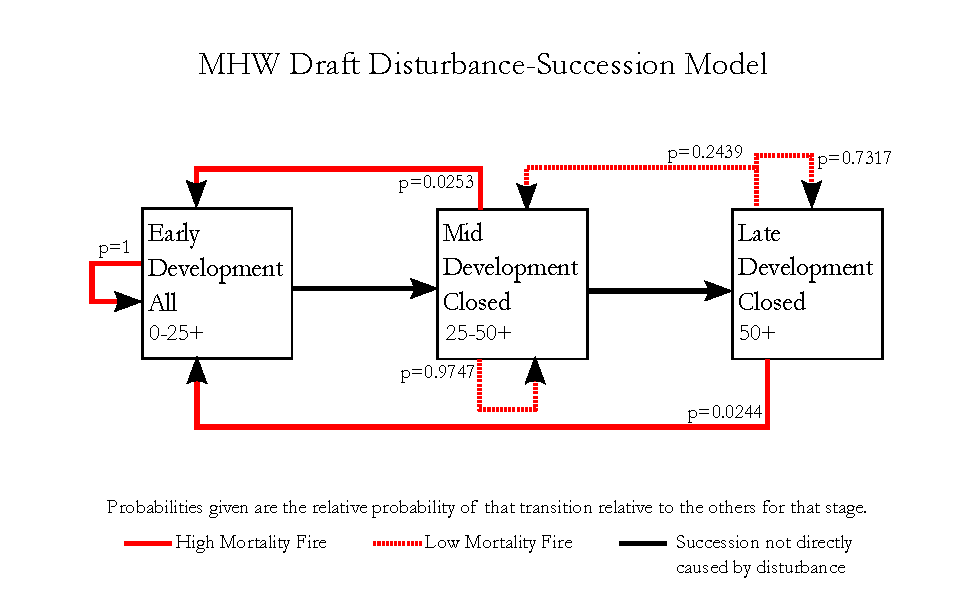
\includegraphics[width=\textwidth]{MHW_Draft_1.pdf}
\end{figure}


\end{document}











